\documentclass[11pt,a4paper,twoside]{article}
\usepackage[top=2cm, bottom=2cm, left=2cm, right=2cm]{geometry}  % nustatomos paraštės
\usepackage[T1]{fontenc}		% LT raidėms su Helvetica
\usepackage[utf8]{inputenc}		% šriftams
%\def\LTfontencoding{L7x}		% LT raidėms su Times New Roman
%\usepackage[L7x]{fontenc}
\usepackage[lithuanian]{babel}	% sulietuvinimas
\usepackage{graphicx}			% paveikslams
\usepackage{caption}			% paveikslu aprašams
\usepackage{subcaption}			% paveikslu aprašams
\usepackage{amsmath}			% formulėms
\usepackage{amsthm}				% sudėtingoms formulėms
\usepackage{amsfonts}			% matematiniams šriftams
\usepackage{pifont}				% šriftams
\usepackage{gensymb}			% matematiniams simboliams
\usepackage{enumerate}			% numeracijai
\usepackage{float}				% paveikslų ir lentelių pozicionavimui
\usepackage[version=3]{mhchem}	% cheminėms formulėms
\usepackage{multirow}			% lentelėms
\usepackage{lmodern}	    	% kitiem šriftam
\usepackage{afterpage}			% formatavimui
\usepackage{setspace}			% tarpui tarp eilučių
\usepackage{hyperref}			% komanda sukuria nuorodas
\hypersetup{					% nuorodos nespalvinamos
	colorlinks,%
	citecolor=black,%
	filecolor=black,%
	linkcolor=black,%
	urlcolor=black
}

\usepackage[scaled]{helvet}			% Helvetica šrifto paketas
\renewcommand{\familydefault}{\sfdefault} % pagrindinio šrifot pakeitimas į Sans, šiuo atveju Helvetica

\begin{document}
\sloppy					% neleidžia tekstui išlįsti į paraštes


\title{$Z^0$ decay into $\mu^{+}$ and $\mu^{-}$}
\author{Nikolajus Elkana Eimutis \\ Taikomoji fizika, Fizikos fakultetas, Vilniaus Universitetas}
\maketitle

\onehalfspace

\paragraph*{Goal:}
Using LHCb open data measure Z boson mass and other important variables (observables?).


\section{Milestones}

\begin{enumerate}
        \item Data is downloaded and ready for local analysis.
        
        \item Theoretical understanding of how LHCb gathers its data is developed.
        
        \item Theoretical understanding of how two muons arise from two protons is developed.

        \item Pratical skill to write root macros is learned.

        \item The data is filtered in such a manner that there is only one evident peak in the Z boson mass graph.

        \item A boson mass graph is drawn, the data is fitted against appropriate theoretical function.
\end{enumerate}
	
% \thispagestyle{empty}			%opcija nenumeruoti pirmojo psl.
\newpage


\section{Theory}
    \begin{enumerate}
        \item Feynman diagrams

        They are figurative depictions of contributions from interactions between particles, which are described by quantum field theory\cite{Jende_Kobel_Pospiech_Bilow_Pedersen_Ould-Saada_Gramstad}.

        \begin{figure}[H]
            \centering

            \subfloat[\centering Muon-antimuon anihilation\cite{Jende_Kobel_Pospiech_Bilow_Pedersen_Ould-Saada_Gramstad}.]{{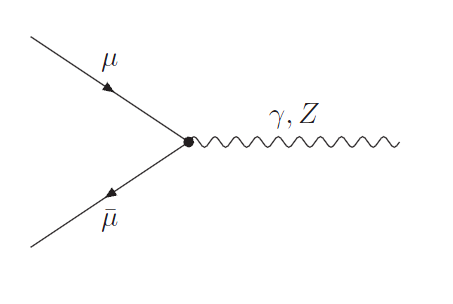
\includegraphics[width=0.5\textwidth]{visuals/002-MuonAntimuonAnihilation.png} }}%
            \subfloat[\centering $Z^0$ decay into muon-antimuon pair\cite{Jende_Kobel_Pospiech_Bilow_Pedersen_Ould-Saada_Gramstad}.]{{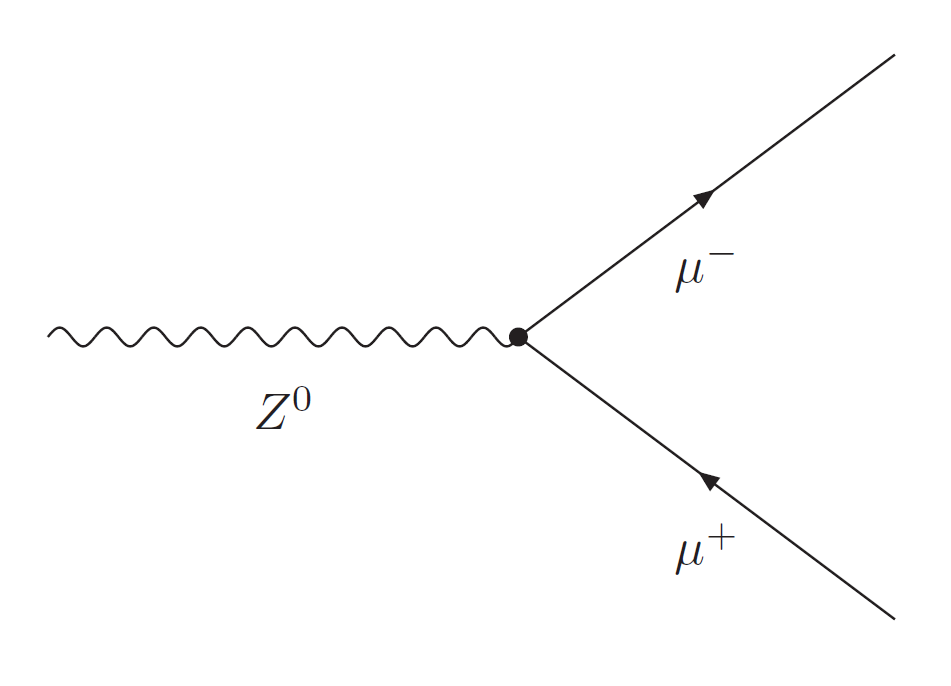
\includegraphics[width=0.5\textwidth]{visuals/001-Z_MyonAntimyon.png} }}%
            
            \caption{Feynman diagrams for the processes with Z boson and muon-antimuon pair.}
            \label{fig:001-Z_MyonAntimyon}
        \end{figure}

        When a quark from one hadron collides with an antiquark of the same flavour form another hadron there is a chance of annihilation. When the net electric charge is zero, they annihilate into virtual photon $\gamma^{*}$ or $Z$ boson\cite{ATLAS_Z_lab}. Due to a short lifetime they soon decay into a pair of leptons. This is so called \textit{Drell-Yan process}.

        \textit{Drell-Yan process} - one of the most important processes that occur in high energy hadron-hadron scattering (for example, proton-proton collisions at LHC). It happens when a quark of one hadron and an antiquark of another hadron annihilate while also creating a virtual photon or $Z$ boson which in turn decays into a pair of oppositely-charged leptons. The energy is almost entirely transformed into mass.

        \begin{figure}[H]
            \centering

            \subfloat[\centering A principal Drell-Yan process diagram\cite{ATLAS_Z_lab}.]{{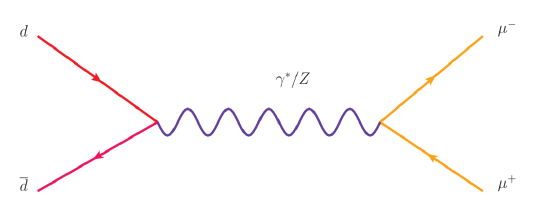
\includegraphics[width=0.5\textwidth]{visuals/003-drell-yan-simple.png} }}%
            \subfloat[\centering A more realistic Drell-Yan process diagram taking into account remnant gluon radiation processes\cite{ATLAS_Z_lab}.]{{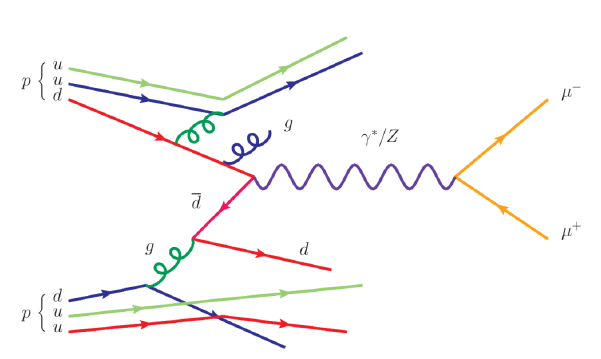
\includegraphics[width=0.5\textwidth]{visuals/004-drell-yan-real.png} }}%
            
            \caption{Feynman diagrams for Drell-Yan processes.}
            \label{fig:002-drell_yan}
        \end{figure}


        \item Processes mimicking $Z$ boson signal

        Due to its short lifetime $Z$ boson is detected by analysing the decay products. Hence, any process producing (in this case) muon-antimuon pair of a mass in the range that we would expect to find the boson would result in a fake signal. It is important to note that the signal can be produced by a bad dimuon candidate, there is no need for a physical process to happen. More on the accuracy and identification efficiency can be found under section 5.


        A few physical processes that produce muons are listed below. Notice that they are of little importance since the produced masses of muons differ vastly from the $Z$ boson decay product. However, single stray muons may induce an error during the $Z$ boson reconstruction stage, if a \textit{Tag and Probe} method was to be used.

        \begin{enumerate}
            \item \textit{pion decay}
            \item \textit{W boson decay}
            \item \textit{Cosmic rays}
        \end{enumerate}


        An important phenomenon to consider when analysing $Z$ boson are "fake signals" coming from virtual photons that have high mass as they are practically indistinguishable from the $Z$ boson.

        
        \item Main graphs drawn when analysing Z boson decay into two muons. What properties are usually analysed?


        These are the parameters analysed in a few different research papers:
        \begin{enumerate}
            \item $G_{\mu}$, $\bar{\alpha}$, $m_Z$ \cite{novikov1999theory};
            \item Muon and Z-boson momentum, pseudorapidity \cite{khodaverdian2019accuracy};
            \item Weinberg angle (indicating the strength of the $W^0$ and $B^0$ bosons mixing), pseudorapidity, tracking and identification efficiencies, $Z$ boson mass cross-section width \cite{ATLAS_Z_lab};
            \item Dimuon invariant mass $m_{\mu^{+} \mu^{-}}$ distribution, transverse momentum $p_T$ distribution, cross section, SPD multiplicity $n_{SPD}$ distribution, tracking efficiency, muon identification efficiency \cite{Bursche:2014ltl}.
        \end{enumerate}
        
        \textbf{[TODO: could add explanations on what each of the parameter means]}

        \textbf{[TODO: could write about why $Z$ boson mass is distribution is fitted againt a convolution of a Gauss or Breit-Wigner distribution]}


        \item Theoretical calculation of Z boson mass from two muons.


        Since $Z$ boson through Drell-Yan process decays into dimuon pair with little energy loss, we could approximate its mass to be that of the \textit{invariant mass} of muon pair.

        \textit{Invariant mass} - a variable that is constant in respect to a moving observer; for a particle with energy $E$ and momentum $\vec{p}$ it is defined as:

        \begin{equation}
            m = \frac{1}{c^2} \sqrt{E^2 - p^2c^2}
            \label{eq:001-invariant-mass}
        \end{equation}

        Invariant mass solves the relativistic problem, where both energy $E$ and momentum $\vec{p}$ measurements change depending on how fast the observer is moving. 

        A more rigorous method for calculating the mass of $Z$ boson could probably be deduced from gauge theory / renormalization / QCD \textbf{[TODO: not sure whether I should add more information on this]}

        Born approximation model, Born process [\textbf{[TODO: ???]}] \cite{khodaverdian2019accuracy}

        

        \item LHCb detector structure, trigger, reconstruction, data validity and error.

        In this section if not explicitly specified, all information is taken (practically word-for-word) from \cite{Bursche:2014ltl} - it contains a very good description about everything.

        \begin{figure}[H]
            \centering

            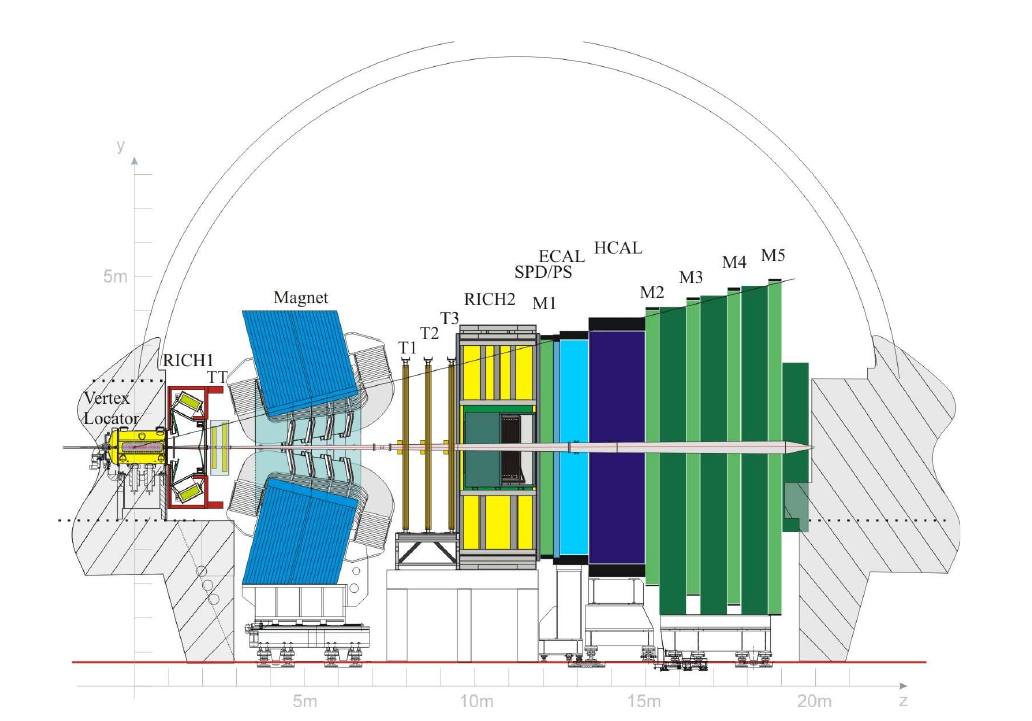
\includegraphics[width=0.7\textwidth]{visuals/005-LHCb-detector.png}
            
            \caption{LHCb detector sketch.}
            \label{fig:001-LHCb_detector}
        \end{figure}

        \begin{figure}[H]
            \centering

            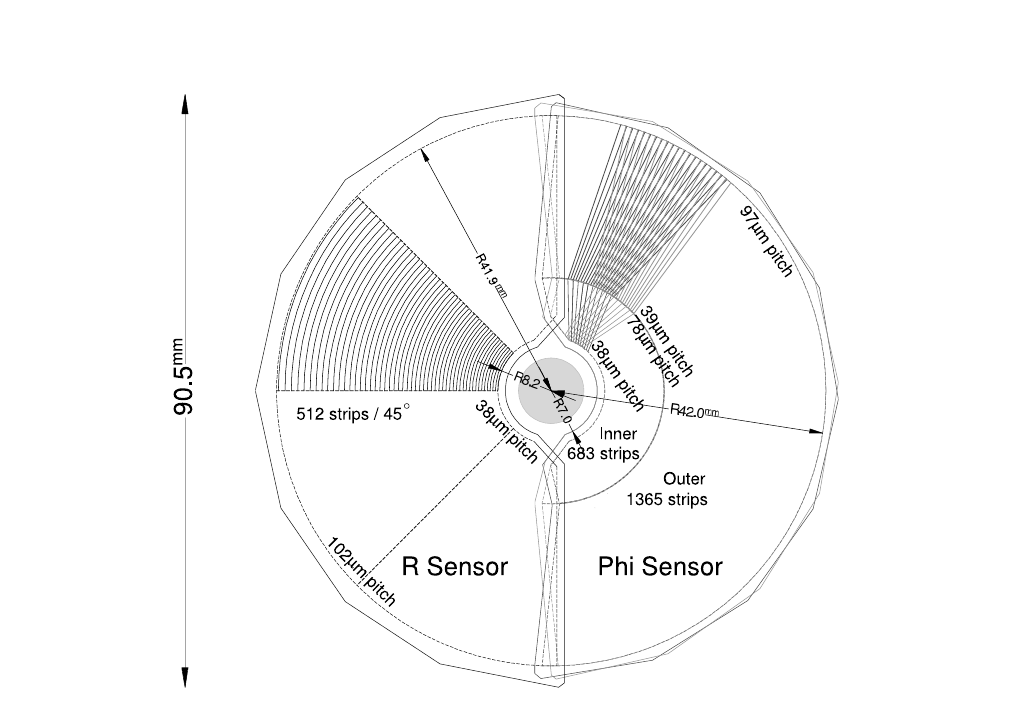
\includegraphics[width=0.7\textwidth]{visuals/006-sensors-in-VeLo.png}
            
            \caption{Sketch of the $r$ and $\phi$ sensors used in VeLo.}
            \label{fig:001-LHCb_detector}
        \end{figure}


        Track types:
        \begin{enumerate}
            \item \textbf{VeLo}
            \item \textbf{backward}
            \item \textbf{upstream}
            \item \textbf{T}
            \item \textbf{downstream}
            \item \textbf{long}
            \item \textbf{$\mu$ stubs}
            \item \textbf{$\mu$ TT}
            \item \textbf{TT}
        \end{enumerate}

        Calorimetry:
        \begin{enumerate}
            \item \textbf{Scintilating pad detector (SPD)}
            \item \textbf{Preshower (PS)}
            \item \textbf{Electromagnetic calorimeter (ECAL)}
            \item \textbf{Hadronic calorimeter (HCAL)}
        \end{enumerate}

        The trigger is organised in three stages:
        \begin{enumerate}
            \item \textbf{L0} - is implemented in hardware and reduces the collision rate from about 20 MHz to 1 MHz.
            \item \textbf{Hlt1} - is executed on standard CPUs.
            \item \textbf{Hlt2} - only logically separated from \textit{Hlt1}. 
        \end{enumerate}



        \begin{figure}[H]
            \centering

            \subfloat[\centering A principal Drell-Yan process diagram\cite{ATLAS_Z_lab}.]{{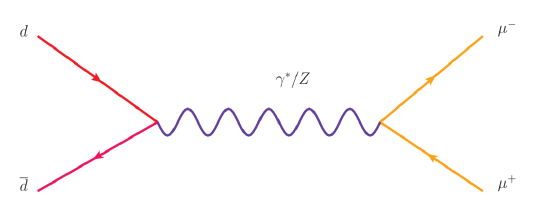
\includegraphics[width=0.5\textwidth]{visuals/003-drell-yan-simple.png} }}%
            \subfloat[\centering A more realistic Drell-Yan process diagram taking into account remnant gluon radiation processes\cite{ATLAS_Z_lab}.]{{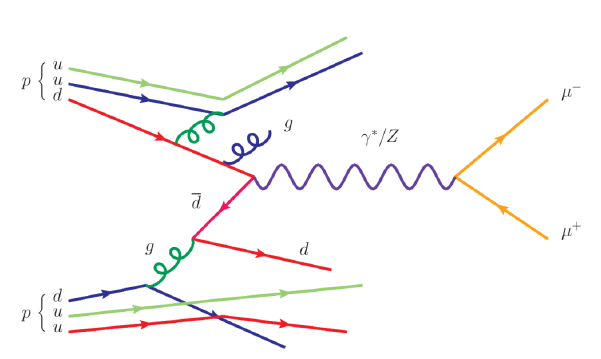
\includegraphics[width=0.5\textwidth]{visuals/004-drell-yan-real.png} }}%
            
            \caption{Feynman diagrams for Drell-Yan processes.}
            \label{fig:001-Z_MyonAntimyon}
        \end{figure}
        
        


        \textit{Tag and probe method} - one well reconstructed and identified muon is combined with a partially reconstructed respectively identified object to a $Z \longrightarrow \mu^{+} \mu^{-}$ candidate.

        [\textbf{[TODO: probably could add more copy pasta]}]

        \item Data types used in LHCb.

        \textbf{[TODO: answer]}
        
    \end{enumerate}


\section{Results}
    
\singlespacing
	
	%\phantomsection
	
\bibliographystyle{VUstyle}
\bibliography{mybib}
	
\end{document}
